\documentclass[12pt]{article}

\usepackage{amsmath, microtype, tikz, physics, gensymb}
\usepackage[letterpaper, bottom=1in, top=1in, left=1in, right=1in]{geometry}

\title{Physics Notes 7}
\date{2/15/2023}
\author{Laith}

\begin{document}
\maketitle

\section{Introduction}

$\va{T}$ is the force vector of the rope tugging on the box $M$. 
\begin{figure}[h]
    \centering
    \begin{tikzpicture}
        \draw (0, 0) -- (0, 2) -- (2, 2) node[midway, yshift=-30] {$M$} -- (2, 0) -- (0, 0);
        \draw[-stealth] (2, 2) -- (4, 4) node[right] {$\va{T}$};
        \draw[dashed] (1, 2) -- (5, 2);
        \draw (2.5, 2.5) arc (50:-12:0.5) node [midway, xshift=5, yshift=2] {$\theta$};
    \end{tikzpicture}
\end{figure}

\noindent With what acceleration should the box be 
moving so that it comes off the ground?

\newpage
\section{Notes}
\begin{itemize}
    \item Tension: is constant through the rope.
    \item It points to the inside of the rope.
\end{itemize}

\begin{figure}[h]
    \centering
    \begin{tikzpicture}
        \draw[very thick] (0, 0) -- (6, 0);
        \draw (3, 0) -- (3, -2);
        \draw (3, -2) arc (90:540:1);
        \draw[red] (4, -3) -- (4, -5);
        \draw[red] (2, -3) -- (2, -7);
        \draw[blue] (1.5, -7) -- (2.5, -7) -- (2.5, -9) node[midway, xshift=-15] {$M$} -- (1.5, -9) -- (1.5, -7);
        \draw[blue] (3.5, -5) -- (4.5, -5) -- (4.5, -6) node[midway, xshift=-15] {$m$} -- (3.5, -6) -- (3.5, -5);
    \end{tikzpicture} 
\end{figure}
\begin{align}
    &T-Mg = MA \\
    &T-mg = ma \\ 
    &A = -a \\
    &T - mg = M(-a) \Rightarrow T=Mg-Ma \\
\end{align}

\section{Newton's Third Law}
``For every force, there is an equal and opposite reaction.''
\bigskip

\noindent If object $A$ exerts force $\va{F}$ on object $B$, then 
object $B$ also exerts force $-\va{F}$ on object $A$.

\newpage
\subsection{Example Problem}
With what velocity will the boxes move?
\begin{figure}[h]
    \centering
    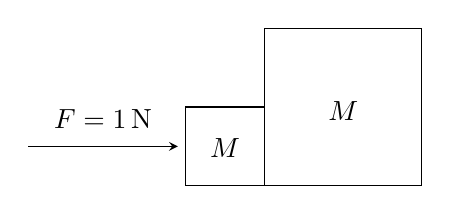
\begin{tikzpicture}
        \draw[-stealth] (-2, 0.5) -- (-0.1, 0.5) node[midway, yshift=10] {$F=1\,\mathrm{N}$};
        \draw (0, 0) -- (0, 1) -- (1, 1) node[midway, yshift=-15] {$M$} -- (1, 0) -- (0, 0);
        \draw (1, 0) -- (1, 2) -- (3, 2) node[midway, yshift=-30] {$M$} -- (3, 0) -- (0, 0);
    \end{tikzpicture}
\end{figure}
\begin{align}
    &F + f = mA
\end{align}


\end{document}